We use a Bayesian approach to model comparison
\cite{Jeffreys1961:Theory-of-Proba,KassRaftery1995:Bayes-Factors,Jaynes2003:Probability-The,VandekerckhoveMatzke2013:Model-Compariso} to find out which
model best explains the observed data. The models under investigation
have unspecified parameters: the speaker's degree of of rationality
$\lambda_\mathrm{S}$, the cost of adjectives $c$, and, for those
listener models that have an action-oriented communication goal, the
listener's degree of rationality $\lambda_\mathrm{L}$. Since there is
no principled theory to determine the value of the parameters, we will
rely mostly on relatively uninformed hyperpriors (so-called to
distinguish them from the salience priors). Based on a specification
of hyperpriors, we calculate the models' \emph{evidences} and compare
them by their \emph{Bayes factors}. The evidence of a model $M$ is the
weighted average of the likelihood of observing the data under all
parameter values:
\begin{align}
  \label{BMA}
  \mathrm{Ev}(M)= \int \Pr(\theta) \cdot \Pr(D | M, \theta)\, \mathrm{d}\theta,
\end{align}
where $\Pr(\theta)$ is the hyperprior over parameter(-tuple) $\theta$
associated with $M$ and $\Pr(D | M, \theta)$ is the likelihood of the
observed data $D$ given the model $M$ and each concrete instantiation
of the parameter(-tuple) $\theta$. The Bayes factor
$K^{M_1}_{M_2}$ is a comparative measure for the plausibility of model
$M_1$ over $M_2$, given their respective hyperpriors and the data in
question:
\begin{align}
  K^{M_1}_{M_2} = \frac{\mathrm{Ev}(M_1)}{\mathrm{Ev}(M_2)} \enspace .
\end{align}
Model $M_1$ makes the data more likely whenever $K^{M_1}_{M_2} > 1$, but
normally only a Bayes factor $K^{M_1}_{M_2} >3$ (or sometimes
$K^{M_1}_{M_2} > 5$) is considered substantial. Values $K^{M_1}_{M_2}
> 10$ are considered strong evidence.

In a sense, comparison by Bayes factors is comparing models in a wider
sense of the term: we actually compare pairs consisting of a model and
its associated hyperprior. For clarity, we refer henceforth to a
model-hyperprior pair as a Model.

\paragraph{Speaker data.} First we look at the speaker models $\sigma_{xy},\
x\in\{a,b\},y\in\{\mathcal{U},\mathcal{S}\}$. Each model has two
parameters $\lambda_\mathrm{S}$ and $c$. We assume that they are
independent of each other:
\begin{equation}\label{hyper-speaker-independent}
\Pr(\lambda_\mathrm{S},c)=\Pr(\lambda_\mathrm{S}) \cdot \Pr(c) \enspace .
\end{equation}
We are uncertain about the rationality of the speaker:
\begin{equation}\label{hyper-speaker-lambda}
\Pr(\lambda_\mathrm{S})= \mathcal{U}_{(0,11)}(\lambda_\mathrm{S}),
\end{equation}
which is a uniform distribution over $(0,11)$. Excluding
$\lambda$-values $\ge 11$ serves practical purposes only, but is
innocuous since the regions of non-negligible posterior likelihood of
$\lambda$ lie safely in the chosen interval for all models. Next, to
allow for the possibility of speaker preferences (nouns over
adjectives or vice versa), we consider two types of hyperpriors for
costs $c$. The first hyperprior has $\Pr(c)= \delta(c)$, the Dirac
delta distribution, that assigns all probability mass $1$ to
$c=0$. This captures the assumption that there is no speaker
preference. The second hyperprior is $\mathcal{U}_{(-0.4,0.4)}$, which
captures the notion that a preference exists, without commitment to
either direction. We restrict our attention to the interval
$(-0.4,0.4)$, because we consider higher levels of cost implausible,
given that utilities for successful communication live in $[0,1]$ and
that we believe that strive for communicative success should outrank
preference satisfaction in a rational model of communication. Taken
together, there are four speaker models, two hyperpriors for each, so
that we compare eight Models with respect to their evidences.

Evidences of speaker Models were calculated by grid approximation. The
results are shown as log-evidences in Table \ref{table:speaker
  mod}. (Notice that the Bayes factor between models is easily
compared by taking the differences between log-evidences.) We can see
that the data very strongly supports speaker models that do not take
the listener's perceptual salience into account. Also, it seems that
action-oriented models are slightly better than their belief-oriented
counterparts, even though the relevant Bayes factors are not
substantial by common standards. Finally, our data makes each speaker
Model that does allow for a speaker preference strongly more plausible
than its counterpart that does not. A look at the posterior likelihood
of $c$ for each speaker model informs us that our data supports the
belief in a speaker preference for nouns, see
Figure~\ref{fig:cost_post_s}. \todo{improve plot}
%
\begin{table}[htb] 
  \centering 
  \caption{Log-evidences of speaker Models. The darker a cell's
    background the higher the evidence.}
  \begin{tabular}{lcccc}
    support of $P(c)$ 
    & $\sigma_{\mathrm{b}\mathcal{U}}$
    & $\sigma_{\mathrm{a}\mathcal{U}}$
    & $\sigma_{\mathrm{b}\mathcal{S}}$
    & $\sigma_{\mathrm{a}\mathcal{S}}$
    \\ \midrule
    $[0,0]$
    & \cellcolor{lightgray!72} -67.48 
    & \cellcolor{lightgray!72}  -67.81 
    & \cellcolor{lightgray!43} -104.14 
    & \cellcolor{lightgray!0} -157.75
    \\
    $(-0.4,0.4)$
    & \cellcolor{lightgray!100} -32.92 
    & \cellcolor{lightgray!99} -33.15  
    & \cellcolor{lightgray!61} \textcolor{lightgray!61}{1}-81.44 
    & \cellcolor{lightgray!15} -139.27
  \end{tabular} 
  \label{table:speaker mod}
\end{table}
%
\begin{figure}[htb]
  \centering
  \caption{Posterior distributions over costs given the data for each
    speaker model.}
  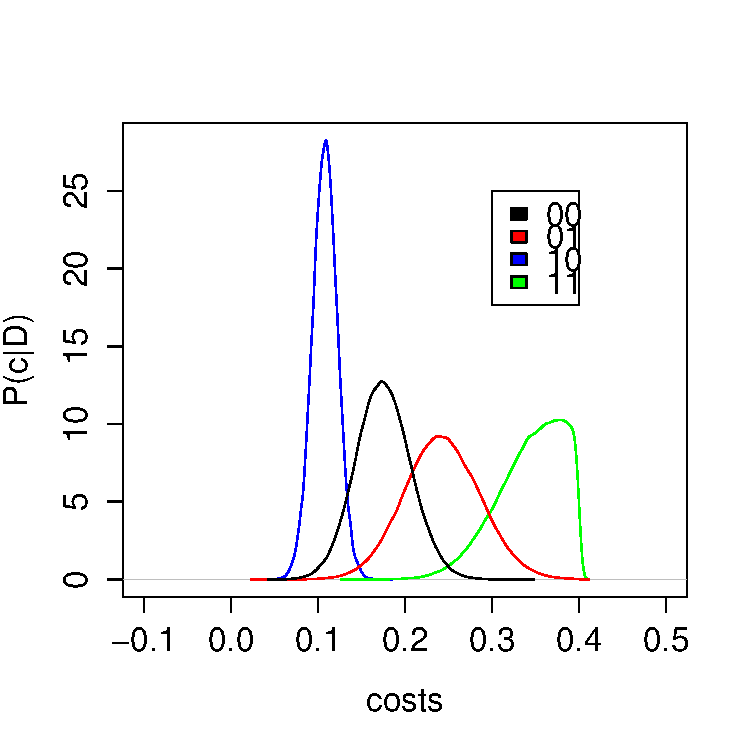
\includegraphics[width=0.5\textwidth]{pics/cost_post_s.pdf}
  \label{fig:cost_post_s}
\end{figure}
%
In sum, our data supports the belief that the speaker does not take
into account the preceptual salience of the listener, while having her
own preference for shape terms over color terms.


\paragraph{Listener data.} Each listener model has a speaker model
nested inside as a belief of the listener about the speaker's
behavior. Section~XYZ \todo{cross-reference} introduced a total of 16
potentially relevant listener models, but we will focus on a selection
only. For one, we restrict our attention to those listener models that
are either entirely belief-based or entirely action-based. In other
words, we exclude as notionally inconsistent models like
$\rho_{\mathrm{a}\cdot}(\sigma_{\mathrm{b}\cdot})$ where the receiver
part assumes an action-based goal structure and the speaker part a
belief-based goal structure. For another, we assume that the
listener's model of the speaker is a reasonable one and therefore put
to the side listener models that embed speaker models that are highly
implausible, given the speaker data as discussed above. Effectively,
this discards listener models that include speaker models that take
the listener's salience prior into account. These two principled
restrictions leave us with four listener models to compare.

Further variation comes from different relevant
hyperpriors. Belief-based models of the listener have the same
parameters as speaker models: the speaker's rationality
$\lambda_\mathrm{S}$ and the speaker's preference costs
$c$. Importantly though, hyperpriors over $\lambda_\mathrm{S}$ and
$c$, although formally parallel to those for speaker models, have a
different interpretation in listener models where they capture our
prior beliefs about the listeners' beliefs about the speakers' likely
rationality and preferences. This is true as well for action-based
models, which also have an additional parameter
$\lambda_\mathrm{L}$. Hyperpriors for the latter encode our prior
beliefs about the listener's actual rationality.

We consider a variety of hyperpriors that differ with respect to
whether they take the speaker's costs into account, whether the
listener's beliefs about the speaker's rationality and preferences are
uninformed (i.e., flat) or informed (i.e., given by the posterior
likelihood of parameters given the actual speaker data) and, in
action-based models, whether the listener's level of rationality
corresponds to his ``informed'' beliefs. The latter option effectively
implements the assumption that there is a tight correlation between
the speaker's actual rationality, the listener's actual rationality
and the listener's beliefs about the speaker's rationality.

Concretely, we consider the following ``flat'' hyperpriors:
\begin{align*}
  \Pr(\lambda_\mathrm{S},c) & =
  \mathcal{U}_{(0,11)}(\lambda_\mathrm{S}) \cdot
  \Pr(c) \\
  \Pr(\lambda_\mathrm{S},c,\lambda_\mathrm{L}) & = 
  \mathcal{U}_{(0,11)}(\lambda_\mathrm{S}) \cdot
    \Pr(c) \cdot  \mathcal{U}_{(0,11)}(
    \lambda_\mathrm{L}),
\end{align*}
for belief-based and action-based models respectively, where $\Pr(c)$
is the hyperprior for the speaker's preference parameter $c$. When
$\Pr(x) = \delta(c)$ we have a hyperprior that does not take costs
into account; otherwise we assume $\Pr(x) =
\mathcal{U}_{(-0.4,0.4)}(c)$, as before.

Hyperpriors that capture the idea that the listener's beliefs are good
guesses of speaker behavior are modeled as if informed by the data
from the speaker experiments:
\begin{align*}
  \Pr(\lambda_\mathrm{S},c) & = \Pr(\lambda_\mathrm{S},c \mid D_\mathrm{S}, M_\mathrm{S}) \\
  \Pr(\lambda_\mathrm{S},c,\lambda_\mathrm{L}) & = 
   \Pr(\lambda_\mathrm{S},c \mid D_\mathrm{S}, M_\mathrm{S}) \cdot  \mathcal{U}_{(0,11)}(
    \lambda_\mathrm{L}) \enspace .
\end{align*}
Here, $D_\mathrm{S}$ is the data from the speaker experiments, and
$M_\mathrm{S}$ the relevant speaker model. For a given listener model,
we consider only the embedded speaker model as relevant. We call
hyperpriors of the above form ``informed'' or, in the case of
action-based models, ``informed uncorrelated''. We distinguish the
latter from ``informed correlated'' hyperpriors of the form:
\begin{align*}
  \Pr(\lambda_\mathrm{S},c,\lambda_\mathrm{L}) & = 
   \Pr(\lambda_\mathrm{S},c \mid D_\mathrm{S}, M_\mathrm{S}) \cdot \Pr(\lambda_\mathrm{L} \mid D_\mathrm{S}, M_\mathrm{S}),
\end{align*}
where the listener's rationality parameter is distributed according to
the relevant posterior. All of the three types of informed hyperpriors
were tested in two varieties: whether the listener takes the sender's
preferences into account or not. If he does not, the posterior
$\Pr(\lambda_\mathrm{S},c \mid D_\mathrm{S}, M_\mathrm{S})$ is derived
from a speaker-hyperprior $\Pr(c) = \delta{c}$; otherwise from $\Pr(c)
= \mathcal{U}_{(-0.4,0.4)}(c)$.

Taken together, we consider two belief-based models, paired with four
hyperpriors, and two action-based models, paired with six hyperpriors
(see Table~\ref{table:listener mod}). Comparing these ten Models is
meant to address the following general questions:
\begin{enumerate}
\item Is the goal structure assumed by participants in our task
  belief-based or action-based?
\item Does the listener take the estimated salience prior into account
  or not?
\item Is the listener's belief in the speaker's level of rationality
  ``correct'', i.e., in line with the observed speaker data?
\item Is the listener's level of rationality related to the speaker's
  actual level of rationality?
\end{enumerate}

Answers to these questions can be found by comparing the evidences of
the Models listed in Table~\ref{table:listener mod}.
%
\begin{table}[htb] 
\caption{Log-evidences for listener Models}
  \centering 
  \begin{tabular}{lccccc}
    prior type & costs &
    $\rho_{\mathrm{b}\mathcal{U}}(\sigma_{\mathrm{b}\mathcal{U}})$ 
    & $\rho_{\mathrm{b}\mathcal{S}}(\sigma_{\mathrm{b}\mathcal{U}})$
    & $\rho_{\mathrm{a}\mathcal{U}}(\sigma_{\mathrm{a}\mathcal{U}})$
    & $\rho_{\mathrm{a}\mathcal{S}}(\sigma_{\mathrm{a}\mathcal{U}})$
    \\ \midrule
    flat
    & no
    & \cellcolor{lightgray!76}{-24.83}
    & \cellcolor{lightgray!94}{-11.66} 
    & \cellcolor{lightgray!77}{-24.06} 
    & \cellcolor{lightgray!75}{-10.62} 
    \\ 
    flat
    & yes
    & \cellcolor{lightgray!76}{-24.80} 
    & \cellcolor{lightgray!96}{-9.84}
    & \cellcolor{lightgray!77}{-23.84}
    & \cellcolor{lightgray!95}{-10.81}
    \\ \addlinespace[0.1cm]
    informed
    & no
    & \cellcolor{lightgray!30}{-59.87} 
    & \cellcolor{lightgray!95}{-10.44}
    & \cellcolor{lightgray!75}{-25.42}
    & \cellcolor{lightgray!98}{-8.48}
    \\
    informed
    & yes
    & \cellcolor{lightgray!18}{-68.43}
    & \cellcolor{lightgray!91}{-13.35}
    & \cellcolor{lightgray!77}{-24.21}
    & \cellcolor{lightgray!93}{-11.85}
    \\ \addlinespace[0.1cm]
    informed-correlated
    & no
    & NA
    & NA
    & \cellcolor{lightgray!23}{-64.70} 
    & \cellcolor{lightgray!100}{-6.80}
    \\
    informed-correlated
    & yes
    & NA
    & NA
    & \cellcolor{lightgray!0}{-82.36} 
    & \cellcolor{lightgray!71}{-29.01}
    \\
  \end{tabular}
  \label{table:listener mod}
\end{table}

The most striking contrast is that models that do not take the
salience prior into account fare much worse than those that do. The
data makes a total rejection of models that rely on uninformative
salience priors strongly plausible.

Another eye-catching feature is that there is a clear winner in the
list. The single best Model, which is substantially better than all
the others, is action-oriented and takes perceptual salience into
account. It has an informed-correlated hyperprior and assumes that the
listener does not take the speaker's preferences into account. This
result is highly thought-provoking, but should be taken with a grain
of salt. It might be that we merely got lucky by restricting the range
of $\lambda_\mathrm{S}$ and $\lambda_\mathrm{L}$ just to a small
region of reasonably high posterior likelihood for these
parameters. Further experimentation should tell us whether
informed-correlated hyperpriors are good predictors in general.

Most generally reliable are the results from flat hyperpriors. Here it
is interesting to note that all of the models that take salience
priors into account, with the exception of
$\rho_{\mathrm{b}\mathcal{U}}(\sigma_{\mathrm{b}\mathcal{S}})$ are
equally plausible, by common standards of Bayes factor
comparisons. This is despite the fact that action-based models have an
additional parameter. It seems that this parameter does not do harm,
but does help to accommodate the assumption that the listener takes
the speaker's preferences into account. 

Action-based models are also better at accommodating the idea that the
listener's estimate of the speaker behavior is roughly correct. The
belief-based models are substantially or strongly less plausible in
this case. In other words, action-based models, possibly due to the
added flexibility of another parameter, are better at explaining
production and comprehension data in unison.

This latter point is of interest with respect to the findings of Frank
\& Goodman that a single parameter choice $\lambda=1$ provided a good
fit for both production and comprehension data. The
rational-speech-act model
$\rho_{\mathrm{b}\mathcal{U}}(\sigma_{\mathrm{b}\mathcal{S}})$ with
fixed parameter $\lambda=1$ is a very poor predictor of our data. (We
focus here on comprehension, but the same applies to production data.)
Assuming $\lambda =1$ as the null hypothesis of a nested-model
comparison, we can use the Savage-Dickey method to compute a Bayes
factor
\cite{DickeyLientz1970:The-Weighted-Li,WagenmakersLodewyckx2010:Bayesian-hypoth}. Let
$\mathcal{M}$ be the parameterized Model with model
$\rho_{\mathrm{b}\mathcal{U}}(\sigma_{\mathrm{b}\mathcal{S}})$ and a
flat hyperprior, not taking costs into account. Given our data we
should adjust our beliefs in parameter value $\lambda=1$ by the Bayes
factor (computed approximately via MCMC sampling):
\begin{align*}
  K = \frac{P(\lambda=1 \mid D_\mathrm{L} \, , \, \mathcal{M})}{P(\lambda=1
    \mid \mathcal{M})} \approx \frac{1.25\text{e-9}}{8.18\text{e-2}} =
  1.52\text{e-8} 
\end{align*}
where $D_\mathrm{L}$ is the listener data. That means that our data
provides very strong evidence that the null hypothesis $\lambda=1$ is
incorrect.

\bigskip

Combining the model comparison results for both the speaker and the
listener models, it seems that if we treat the speaker's preference as
some lexical salience which together with the listener's perceptual
salience constitutes the contextual salience of the referential game,
then contextual salience actually manifests \emph{lack of} common
knowledge between the speaker and the listener rather than the
presence of it, since they both have some preference that biases their
decisions but they are unaware of each other's such
preference. However, there is indeed something common between the
speaker and the listener, i.e. the distribution of the degree of
rationality. Also, the listener's belief about the speaker is correct
modulo the speaker's private lexical salience.


%%% Local Variables: 
%%% mode: latex
%%% TeX-master: "main"
%%% TeX-PDF-mode: t
%%% End: